\section{SISTEMA DE SOFTWARE DO FUTEBOL DE ROB{\^O}S}

O sistema deste time pode ser representado
simplificadamente atrav{\'e}s do diagrama apresentado na Fig. 2
que indica as partes principais do processamento. Estas partes
s{\~a}o descritas, juntamente com as intera{\c c}ões entre elas, na
sequ{\^e}ncia. A C{\^A}MERA captura uma imagem do campo que {\'e}
digitalizada por uma placa espec{\'i}fica. Esta imagem {\'e} processada pelo m{\'o}dulo de 
VIS{\~A}O que determinar{\'a} as posi{\c c}{\~o}es atuais dos rob{\^o}s a partir de suas etiquetas coloridas 
e a da bola que possui cor alaranjada. A PREVIS{\~A}O, com base das informações recebidas do m{\'o}dulo da
VIS{\~A}O, define as posi{\c c}{\~o}es mais prov{\'a}veis que os objetos em campo ir{\~a}o 
assumir alguns instantes a frente. Com estas posi{\c c}{\~o}es (presente e futura). O m{\'o}dulo de
ESTRAT{\'E}GIA calcula os locais do campo que os rob{\^o}s do time controlado dever{\~a}o se posicionar. 
Para realizar estes c{\'a}lculos, este m{\'o}dulo faz uso de roteiros, que são específicos para cada rob{\^o}.
Basicamente, um roteiro {\'e} um conjunto de comportamentos espec{\'i}ficos para cara rob{\^o} que faz com que
este assuma uma postura defensiva ou ofenciva durante uma partida. O m{\'o}dulo de CONTROLE, fazendo uso das 
posi{\c c}{\~a}o atuais de cada rob{\^o} (VIS{\~A}O) e de seus objetivos (ESTRAT{\'E}GIA), determina maior
velocidade poss{\'i}vel que um rob{\^o} pode assumir para que este consiga chegar ao seu objetivo e parar,
definindo os valores de cada roda a serem enviados aos rob{\^o}s via r{\'a}dio, fazendo os rob{\^o}s se moverem 
para concluir a estrat{\'e}gia. Todos estes m{\'o}dulos s{\~a}o executados no computador pessoal.

% FIGURA 2
\begin{figure}[!htb]
\centering
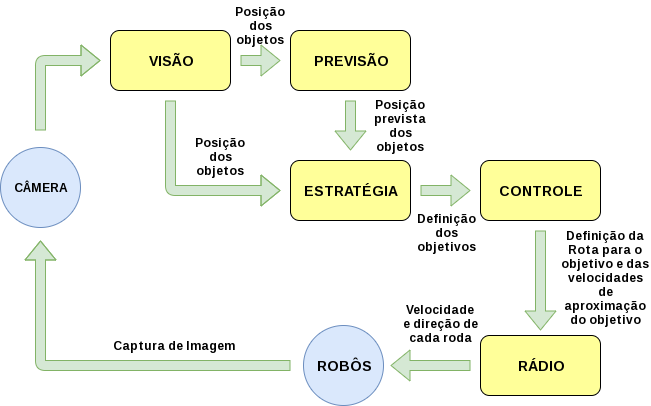
\includegraphics[width=240pt, height=160pt]{novo_carrosselTDP.png}
\caption{Diagrama simplificado dos m{\'o}dulos do time Carrossel Caipira.}
\label{Rotulo}
\end{figure}
%%%

\subsection{M{\'o}dulo da Vis{\~a}o}

No ambiente de futebol de rob{\^o}s toda a estrat{\'e}gia e o
controle, tanto de baixo n{\'i}vel quanto de alto n{\'i}vel, s{\~a}o
baseados na interpreta{\c c}{\~a}o das imagens captadas pela c{\^a}mera.
Para que isso seja realizado, etiquetas de cores em destaque
localizadas no topo dos rob{\^o}s identificam cada um deles, em
rela{\c c}{\~a}o a seu time e possivelmente sua fun{\c c}{\~a}o, conforme
demonstra a Fig. 3.

O tempo de execu{\c c}{\~a}o do ciclo de controle do sistema foi
definido pela taxa de aquisi{\c c}{\~a}o de imagens. Como o time
Carrossel Caipira usa c{\^a}meras de v{\'i}deo convencionais, a taxa {\'e}
limitada a 30 quadros por segundo. Portanto, a cada per{\'i}odo de
33 ms, uma nova imagem refletindo o estado atual do campo
torna-se dispon{\'i}vel ao computador para processamento. Cada
uma dessas imagens {\'e} capturada e digitalizada por uma placa
de captura, que disponibiliza, na forma de uma matriz com
dimensões 640x480 pixels com tr{\^e}s canais (componentes Red,
Green, Blue - RGB). Cada um desses pixels deve ser analisado,
quanto a sua cor, para identificar se {\'e} uma cor de import{\^a}ncia
ao sistema, esta t{\'e}cnica {\'e} chamada de segmenta{\c c}{\~a}o de cor.

% FIGURA 3
\begin{figure}[!htb]
\centering
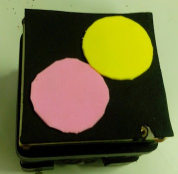
\includegraphics[scale=0.9]{etiqueta.png}
\caption{ Etiqueta de identifica{\c c}{\~a}o do rob{\^o}}
\label{Rotulo}
\end{figure}
%%%

\subsection{M{\'o}dulo de Estrat{\'e}gia}

A estrat{\'e}gia {\'e} o m{\'o}dulo respons{\'a}vel por definir a meta de
cada rob{\^o}. Utilizando as coordenadas atuais e previstas da bola, dos
rob{\^o}s do time e dos advers{\'a}rios este m{\'o}dulo decide qual {\'e} a posi{\c c}{\~a}o 
mais indicada para cada rob{\^o} do time, de tal forma que corresponda ao comportamento que
os rob{\^o}s devem desempenhar na partida. No caso do time Carrossel Caipira
tem-se tr{\^e}s tipos de comportamentos: goleiro, defensor e
atacante.

{\bf Goleiro}: O rob{\^o} {\'e} posicionado na proje{\c c}{\~a}o da posi{\c c}{\~a}o da
bola com a linha defensiva do gol, se a bola vir diretamente na
dire{\c c}{\~a}o da regi{\~a}o do gol. Caso contr{\'a}rio o rob{\^o} se alinha com a
bola na coordenada y do sistema, dessa forma sempre permanecendo em
frente ao gol. Para permitir que o posicionamento seja r{\'a}pido, o rob{\^o} deve
manter sua orienta{\c c}{\~a}o em 90 ou 270 graus, como {\'e} mostrado
na Fig. 4.

% FIGURA 4
\begin{figure}[!htb]
\centering
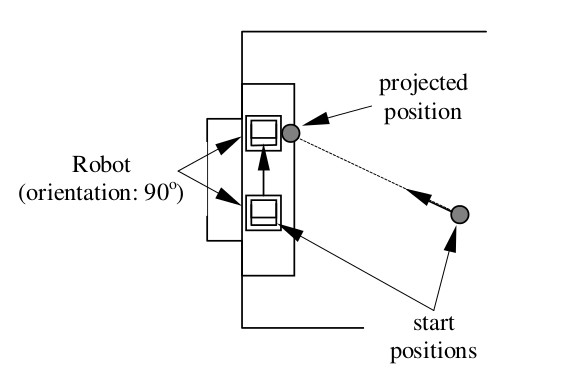
\includegraphics[scale=0.5]{pos_goleiro.png}
\caption{Comportamento do goleiro. Fonte: Costa et al. [3].}
\label{Rotulo}
\end{figure}
%%%

{\bf Volante}: O rob{\^o} {\'e} posicionado na dire{\c c}{\~a}o da coordenada y
da bola, bloqueando a bola e impedindo seu avan{\c c}o at{\'e} o gol.
Mas deve permitir a bola passar se ela estiver sendo conduzida
pelo atacante. Quando o volante e a bola est{\~a}o em situa{\c c}{\~a}o
favor{\'a}vel no que diz respeito a um poss{\'i}vel ataque ao gol
advers{\'a}rio, ele troca de comportamento com o atacante e tenta
atacar. A situa{\c c}{\~a}o favor{\'a}vel acontece quando o defensor
estiver pr{\'o}ximo da bola em posi{\c c}{\~a}o de ataque.

{\bf Atacante}: Nesta posi{\c c}{\~a}o existem dois tipos de
comportamento: (i) modo de posicionamento: quando o
objetivo {\'e} posicionar o rob{\^o} atr{\'a}s da bola para bloquear algum
advers{\'a}rio ou deixar o rob{\^o} apto para trocar seu modo; (ii)
modo de condu{\c c}{\~a}o, quando o rob{\^o} empurra a bola at{\'e} o gol.

Atrav{\'e}s destes comportamentos {\'e} calculada a posi{\c c}{\~a}o que o
rob{\^o} deve atingir, ou seja, as coordenadas x, y e o {\^a}ngulo que o
rob{\^o} deve alcan{\c c}ar para realizar a estrat{\'e}gia espec{\'i}ficada por seu roteiro.
Esta posi{\c c}{\~a}o {\'e} importante para o m{\'o}dulo de Controle, no que se
refere ao planejamento do caminho {\'o}timo, pois define o fim do
trajeto (o objetivo) escolhido por ele, bem como o {\^a}ngulo desejado de chegada, permitindo
calcular a forma como o rob{\^o} deve chegar l{\'a}.

\subsection{M{\'o}dulo de Controle}

A partir das coordenadas detectadas pelo m{\'o}dulo de Vis{\~a}o
e das coordenadas atribu{\'i}das pelos resultados do m{\'o}dulo de
Estrat{\'e}gia, o m{\'o}dulo de Controle deve determinar as melhores
trajet{\'o}rias e comandos a ser enviados aos rob{\^o}s.

O c{\'a}lculo de uma trajet{\'o}ria deve levar em conta o desvio de
obst{\'a}culos, evitando os outros rob{\^o}s na arena. Este c{\'a}lculo {\'e}
necess{\'a}rio para levar o rob{\^o} da sua posi{\c c}{\~a}o atual at{\'e} a
determinada pela estrat{\'e}gia. No caso do time Carrossel Caipira,
{\'e} empregado um m{\'e}todo chamado de campo potencial. Os
campos potenciais partem da ideia de for{\c c}as imagin{\'a}rias
atuando sobre o rob{\^o}, ideia proposta por Khatib [4], na qual a
''for{\c c}a causada'' pelos obst{\'a}culos {\'e} de car{\'a}ter repulsivo e pela
meta, de car{\'a}ter atrativo. Por{\'e}m a interfer{\^e}ncia das ''for{\c c}as''?
geradas a partir de v{\'a}rios obst{\'a}culos podem produzir locais
{\'o}timos que atrapalham o desempenho do sistema para
encontrar um caminho at{\'e} a meta para o rob{\^o}.

Para evitar esta situa{\c c}{\~a}o, Connoly et al. [5] solucionaram
o problema utilizando fun{\c c}ões harm{\^o}nicas para o c{\'a}lculo do
campo potencial de ambientes nos quais as posi{\c c}ões das
paredes, objetos e metas sejam conhecidas, que {\'e} o caso do
ambiente de futebol de rob{\^o}s. As fun{\c c}ões harm{\^o}nicas
utilizadas s{\~a}o solu{\c c}ões para a equa{\c c}{\~a}o de Laplace (1).
\begin{equation}
\nabla = 0 \ para \ P : R \rightarrow R .
\end{equation}

Assim {\'e} definido um Problema de Valor de Contorno na
regi{\~a}o de atua{\c c}{\~a}o do rob{\^o} utilizando a condi{\c c}{\~a}o de Dirichlet%
\footnote{A condição de contorno de Dirichlet (ou de primeiro tipo) é um tipo
de condição de contorno, nomeada em homenagem a Johann Peter
Gustav Lejeune Dirichlet (1805-1859). Quando aplicada sobre uma
equação diferencial ordinária ou parcial, especifica os valores que uma
solução necessita para tomar-se sobre o contorno do domínio
}
com potencial alto para obst{\'a}culos e potencial baixo para a
meta. Ent{\~a}o, s{\~a}o extra{\'i}das as linhas de for{\c c}a, com base no
gradiente descendente [5][6] do potencial, que direcionam o
rob{\^o} para sua meta, desviando-o de obst{\'a}culos.

Uma vez obtido o campo potencial, tem-se o {\^a}ngulo ideal
que o rob{\^o} deve atingir para se deslocar at{\'e} a meta, que
chamamos de {\^a}ngulo objetivo, basta agora calcular a dire{\c c}{\~a}o e
velocidade de cada motor. 
